\documentclass[12pt, a4paper]{article}
\usepackage{amsmath, amsfonts}
\usepackage[utf8]{inputenc}
\usepackage[russian]{babel}
\usepackage{graphicx}
\usepackage{tikz}
\usepackage{xcolor}
\usepackage{wrapfig}
\usepackage{float}
\usepackage{geometry}
\usepackage[indentfirst,compact,topmarks,calcwidth,pagestyles]{titlesec}
\usepackage{verbatim}
\usepackage{titletoc}
\usepackage{cmap}
\textheight=24cm
\textwidth=16cm
\oddsidemargin=5mm
\evensidemargin=-5mm
\marginparwidth=36pt
\topmargin=-1cm
\footnotesep=3ex
\raggedbottom
\tolerance 3000
\clubpenalty=10000
\widowpenalty=10000
\usepackage[T2A]{fontenc}
\usepackage{hyperref}
\usepackage{psfrag}

\newcommand\todo[1]{\marginpar{\textcolor{red}{#1}}}

\DeclareMathOperator*{\argmax}{argmax}
\DeclareMathOperator{\weight}{weight}
\DeclareMathOperator{\score}{score}
\DeclareMathOperator{\simu}{sim}
\DeclareMathOperator{\Dir}{Dir}
\DeclareMathOperator{\DP}{DP}
\DeclareMathOperator{\svert}{\,\vert\,}

\usepackage[ruled, linesnumbered]{algorithm2e}
\SetKwInput{KwData}{Исходные параметры}
\SetKwInput{KwResult}{Результат}
\SetKwInput{KwIn}{Входные данные}
\SetKwInput{KwOut}{Выходные данные}
\SetKwIF{If}{ElseIf}{Else}{если}{тогда}{иначе\ если}{иначе}{конец\ условия}
\SetKwFor{While}{до\ тех\ пор,\ пока}{выполнять}{конец\ цикла}
\SetKw{KwTo}{от}
\SetKw{KwRet}{возвратить}
\SetKw{Return}{возвратить}
\SetKwBlock{Begin}{начало\ блока}{конец\ блока}
\SetKwFor{For}{цикл}{выполнять}{конец\ цикла}
\SetKwFor{ForEach}{для\ каждого}{выполнять}{конец\ цикла}
\SetKwRepeat{Repeat}{повторять}{до\ тех\ пор,\ пока}
\SetAlgorithmName{Алгоритм}{алгоритм}{Список алгоритмов}

%\usepackage{titlesec}
%\newcommand{\sectionbreak}{\clearpage}

%\psfrag{all-freq-x}{день}
%\psfrag{topic-specific}{тематические}

\begin{document}

Титульный лист\thispagestyle{empty}\newpage

\tableofcontents\thispagestyle{empty}\newpage

  \section{Введение}
  	В современном мире информация быстро устаревает, поэтому способы вовремя находить нужные данные --- постоянный объект для исследований. Одним из направлений в этой области является извлечение данных из платформ микроблогов.
  	
  	Платформы микроблогов стали очень популярным способом размещения данных в Сети. В них можно найти сообщения пользователей практически на любую тему, начиная стихийными бедствиями и заканчивая рейтингами музыкальных исполнителей. Правильная обработка доступной информации --- нетривиальная задача, которая имеет множество областей применения. Последние несколько лет эта тема активно исследуется во многих университетах мира.
  	
	Отслеживание сообщений о стихийных бедствиях в реальном времени поможет вовремя организовать спасательные операции и сохранить жизни людей\cite{nuggets}. Руководствуясь сообщениями пользователей микроблогов можно судить о популярности товаров и вовремя принимать экономически целесообразные решения. Можно делать предположения о рейтингах политических деятелей и эффективности рекламы на основании информации в микроблогах. Помимо перечисленных способов применения доступной информации в микроблоггинговых платформах можно привести множество других.
	
	В данной работе в дальнейшем будет рассматриваться сервис микроблогов Твиттер\footnote{http://www.twitter.com}. В нем помимо текстовой информации можно публиковать фото, видео и геотеги, что так же может быть использовано при анализе, но в этой работе не рассматривается. В доступном наборе данных можно проводить анализ разных сущностей, эта работа посвящена выявлению событий среди потоков информации. Поскольку трактовка событий в сообщениях микроблогов может быть субъективной, выделим несколько свойств, которыми характеризуется событие.
	
	Событие в первую очередь должно быть чем-то аномальным на фоне остальных данных. Оно определяется резким изменением частотных характеристик некоторых слов в сообщениях. События в микроблогах носят взрывной характер, в течении нескольких часов частоты релевантных слов возрастают в десятки раз и так же быстро опускаются до нормального уровня. Примером события могут быть: стихийное бедствие, выход законопроекта на резонансную тему, получение фильмом награды на кинофестивале.
	
	Существуют разные подходы для решения описанной задачи. В следующих двух разделах будут даны формальные определения и рассмотрены некоторые подходы для решения задачи извлечения событий.
	
  \section{Описание задачи}
	Цель дипломной работы состоит из нескольких частей:
\begin{itemize}
\item исследовать существующие подходы по извлечению событий из сообщений пользователей, выделить возникающие проблемы и рассмотреть возможные методы их решения,
\item исследовать возможность применения тематических моделей для решения задачи выявления событий,
\item разработать метод для извлечения событий из сообщений пользователей сети Твиттер на основе иерархического процесса Дирихле,
\item протестировать работу алгоритма на реальных данных.
\end{itemize}	  
  
  Объект изучения этой работы --- алгоритм, который по входным данным строит множество событий. В качестве данных для задач подобного рода служит корпус документов (сообщений):
\begin{equation}
  \Omega = \left\{D_i \svert i \in \overline{1,n} \right\}.
  \end{equation}  
  Будем считать, что каждый документ $D_i$ имеет временную метку $t_i$. В свою очередь документ $D_i$ определяется как упорядоченный набор слов:
\begin{equation}
  D_i = \left\{w_j \svert j \in \overline{ 1, l_i } \right\},
  \end{equation}  
   при этом слова в документах принадлежат некоторому словарю $V$. 
  
  Событие --- некоторая сущность, которая характеризуется временем возникновения и ключевыми словами. Оно вызывает резкий подъем частотных характеристик некоторых слов. Событием может быть футбольный матч и музыкальный концерт. В социальной сети Твиттер есть популярные темы, которые всегда генерируют много сообщений. Например это сообщения с ключевыми словами iphone и ipad. Но такие сообщения нельзя считать событиями. Также событиями нельзя считать еженедельные пятничные сообщения о конце рабочей недели\cite{waim13}.
  
  Особенности социальной сети Твиттер состоят в следующем:
  \begin{itemize}
  \item короткие сообщения (до 140 символов),
  \item наличие шума и ошибок,
  \item большая плотность сообщений,
  \item ``взрывной'' характер событий.
  \end{itemize}
  
  \section{Анализ существующих подходов}
  Прежде чем составлять решение задачи были изучены существующие подходы. Все они комбинируют техники машинного обучения, обработки текстов, вероятностных графических моделей и других разделов науки. Разные методы лучше работают для одних данных и хуже для других, на их качество также влияет природа данных. Выделим несколько подходов, для того чтобы изучить общую схему подобных алгоритмов и чтобы обозначить идеи, которые могут быть использованы при составлении метода извлечения событий из сообщений сети Твиттер.
  
%  \todo{сделать введение и заключение к каждому методу}
  
  \subsection{NED}
  \label{ned-subsection}
	Исторически первым подходом к извлечению событий принято считать NED (New Event Detection)\cite{ned}. NED предназначен для того, чтобы находить первый документ на тему, которая не встречалась раньше. Следующие документы на эту тему уже не будут новыми и не будут помечены алгоритмом. Для того, чтобы отвечать на вопрос, является ли документ новым, необходимо указать способ как определять степень сходства двух документов.
	
\begin{figure}[H]
  \centering
  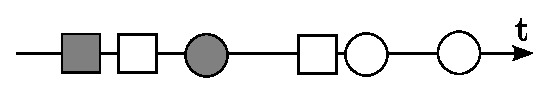
\includegraphics[width=0.58\textwidth]{ned.eps}
  \\
  \caption{Документы, соответствующие двум разным темам. Новые документы помечены серым цветом.}
  \end{figure}  

	Для этого в алгоритме NED используется техника Incremental TF--IDF (Term Frequency -- Inverse Document Frequency). TF--IDF --- базовый метод выяснять насколько отдельно взятые слова характеризуют весь документ, другими словами, насколько большой вес имеет слово $w$ в документе $d$. Пусть $f(d,w)$ --- количество слов $w$ в документе $d$. Определим значение $df_t(w)$ как количество документов, поступивших не позднее времени $t$, в которых встречается слово $w$. Используя введенные величины, можно записать значение веса определенного слова $w$ в документе $d$. В момент времени $t$ имеем:
	\begin{equation}
	\weight_t(d,w) = \frac{1}{Z_t(d)}f(d,w) \cdot \log \frac{N_t}{df_t(w)},
	\end{equation}
	где $N_t$ --- общее количество документов, поступивших не позднее времени $t$, $Z_t(d)$ --- нормализационное значение:
	\begin{equation}
	Z_t(d) = \sqrt{\sum_w \left[ f(d,w) \cdot \log \frac{N_t}{df_t(w)} \right]^2}.
	\end{equation}.
	
	Теперь можно записать значение похожести двух документов, $q$ и $d$:
	\begin{equation}
	\simu_t(d,q) = \sum_w \weight(w, d) \cdot \weight(w, q).
	\end{equation}
	Указанные формулы записаны в косинусной метрике, также могут быть использованы метрики Хеллингера, Кульбака--Лейблера и другие.
	
	Для того, чтобы понять, является ли добавленный в момент времени $t$ документ $q$ новым, необходимо вычислить степень его похожести со всеми предыдущими документами. Пусть $d^*$ --- документ, максимально похожий на $q$:
	\begin{equation}
	d^* = \argmax_d \simu_t (d,q).
	\end{equation}
	Тогда значение
	\begin{equation}
	\score_t(q) = 1 - \simu_t (d^*, q)
	\end{equation}
	может быть использовано для того, чтобы определить, является ли документ $q$ новым. Новыми будем считать все документы $q$, у которых значение $\score_t(q)$ больше, чем пороговое значение $\theta_s$. В обратном случае считается что существует документ $d^*$, достаточно похожий на $q$ и поэтому $q$ не представляет собой сообщение на новую тему. Для того, чтобы определить подходящее значение $\theta_s$, можно использовать размеченный корпус и посчитать значение $\simu_t (d,q)$ среди документов, соответствующих одному и разным событиям.
	
	Недостатком алгоритма NED является то, что он не учитывает отношения между словами. Например синонимичные слова в NED будут считаться совершенно разными. Для того, чтобы решить эту проблему могут быть применены тематические модели.
	
	\subsection{Выявление событий с помощью LDA}
  На следующем примере рассмотрим как тематические модели (topic models) могут быть использованы для задачи распознавания событий. Для этого опишем схему, по которой работает алгоритм, предложенный в статье \cite{mediaeval}. 
  
  Задача состоит в том, чтобы по данным к  набору фотографий Flickr\footnote{http://www.flickr.com} распознать все события на определенную тему, проходившие в обозначенных городах. Есть несколько вариантов постановок задачи, они различаются тематикой событий и городами. 
  
  Фотографии содержат в себе описания, они будут являться документами в задаче распознования. Также фотографии могут включать геотеги. Авторы статьи предлагают разбить решение задачи на пять составных частей: 
  \begin{enumerate}
  \item предобработка текстовых данных,
  \item определение в каком городе сделана фотография по ее описанию,
  \item распознавание темы, к которой относится фотография,
  \item распознавание события, к которому относится фотография, \label{list:event-extracting}
  \item оптимизация описания события, полученного на шаге \ref{list:event-extracting}.
  \end{enumerate}
  
  В качестве предобработки, авторы предлагают выполнить следующее: удалить стоп-слова и html теги, провести стемминг слов\footnote{стемминг (stemming) --- удаление окончаний у слов для их нормализации}, перевести не английские слова на английский язык используя сервис Google Translate.
  
	Так как задача упоминает отдельные города, необходимо разработать метод распознавания города по документу. Указанные в фотографии географические координаты были доступны авторам в 20\% случаев, из этих координат были выявлены города используя сервис Google Tables. Используя технику TF--IDF, в описаниях фотографий с известными городами были извлечены ключевые слова. По этим ключевым словам появилась возможность назначить фотографиям без геотегов ``ближайший'' город с точки зрения похожести описаний. Для того чтобы определять похожесть документов, был использован подход, описанный в~(\ref{ned-subsection}). В случаях, когда ``ближайший'' город выявить не удавалось, авторами использовались следующие предположения: считалось что один и тот же фотограф не мог побывать в один день более чем в двух разных городах, и что путешествие из одного города в другой занимает как минимум два часа. Эти предположения позволили улучшить классификатор, таким образом более 97\% фотографий были привязаны к городу.
	
	Далее необходимо для каждого города кластеризовать документы по темам и рассмотреть только те из них, которые заданы в описании задачи. Для распознования тем была использована тематическая модель LDA (Latent Dirichlet Allocation)\cite{lda-model}, для определения параметров которой применялось сэмплирование по Гиббсу\cite{lda-gibbs}. LDA работает из предположения, что каждый документ $D_i$ характеризуется случайным распределением над темами, в то время как каждая тема является мультиномиальным распределением над словами.
	
	Оставшаяся часть --- извлечение событий и их оптимизация. Для того, чтобы алгоритм выявил событие, отвечающее теме $k$ в день $d$, необходимо чтобы количество документов $D_i$ по этой теме в день $d$ превосходило некоторое пороговое значение $\theta$. Оптимизация событий подразумевает под собой объединение событий на одну тему в последовательные дни и разделение событий в разных городах.
	
	Авторы статьи тестировали алгоритм на трех разных вариантах условия задачи, в таблице~\ref{lda-table} приведены результаты по каждому из них.
	
\begin{table}[h]
	\centering
    \begin{tabular}{c c c c}
    Данные & Точность & Полнота & F-мера \\ \hline
    \#1 & 80.98 & 19.25 & 31.10 \\ 
    \#2 & 91.21 & 77.85 & 84.00  \\ 
    \#3 & 90.76 & 81.91 & 86.11 \\ \hline
    \end{tabular}
    \caption{Точность, полнота и F-мера алгоритма при разных условиях задачи}
    \label{lda-table}
\end{table}

	По результатам из таблицы можно видеть что в первом случае алгоритм справляется со своей задачей существенно хуже, чем в других. Авторы объясняют это тем, что в задаче \#1 необходимо было находить научные конференции, а так как они проходят на разные темы, не получалось выделить конкретный набор ключевых слов. По этой причине полнота алгоритма в случае \#1 относительно низкая. В задаче \#2, \#3 напротив удалось обозначить необходимые ключевые слова, о чем свидетельствуют результаты.
	
	\subsection{Information nuggets}
	Рассмотрим подход к извлечению событий, описанный в~\cite{nuggets}. Авторы ставят перед собой задачу составить алгоритм описания подсобытий в социальной сети Твиттер. Были использованы данные, полученные во время торнадо Joplin в 2011 году. Данные представляют из себя сообщения пользователей, содержащие хэштег \#joplin, собранные 22 мая 2011 года на протяжении нескольких часов, пока плотность сообщений не стала относительно низкой. Авторы ставили цель извлекать из потока сообщений так называемые золотые самородки информации --- короткие и информативные сообщения, описывающие происходящие события. По этой причине подход назван information nuggets.
	
	Авторы видели основную проблему в том, что даже при наличии большого количества сообщений об одном событии, ими трудно пользоваться, потому что они имеют разную природу. Например это может быть сообщение очевидца о происходящем стихийном бедствии или сообщение о перечислении правительством средств на восстановление разрушенных построек. Статья предлагает делить сообщения на пять разных категорий по степени информативности:
	\begin{itemize}
	\item\emph{Персональное}:
	информация в сообщении может быть полезна только автору и его кругу общения. Она не является интересной для людей, которые не знают автора сообщения непосредственно.
	\item\emph{Информативное (напрямую)}:
	сообщение может быть полезно людям вне круга общения автора, и эта информация написана прямым участником или очевидцем событий.
	\item\emph{Информативное (косвенно)}:
	сообщение может быть полезно людям вне круга общения автора, при этом автор пишет о том, что он слышал по телевидению, радио или любому другому источнику информации.
	\item\emph{Информативное (напрямую или косвенно)}:
	сообщение может быть полезно людям вне круга общения автора, но невозможно ответить на вопрос как автор связан с происходящими событиями.
	\item\emph{Другое}:
	сообщение или не на английском языке, или не может быть классифицировано.
	\end{itemize}
	
	В дальнейшем рассматриваются только сообщения с информативным типом, так как они наиболее вероятно содержат полезные сведения. Затем сообщения разбиваются на подтипы по направленности информации. Всего авторами использовалось 32 разных подтипа, среди которых:
	\begin{itemize}
	\item\emph{Предостережения и советы}: документ содержит предупреждение о возможном опасном происшествии.
	\item\emph{Жертвы и разрушения}: в тексте сообщается о потерях, вызванных стихийным бедствием.
	\item\emph{Сбор средств}: сообщения описывают пожертвования денег и предметов пострадавшим от чрезвычайного происшествия.
	\end{itemize}
	
	Для того, чтобы классифицировать сообщения по типам и подтипам, в алгоритме используется наивный байесовский классификатор, который предварительно тренируется на размеченных данных. В классификаторе используется большое количество свойств, бинарных, скалярных и текстовых. В таблице~\ref{nuggets-table} приведены результаты работы алгоритма на некоторых подтипах. Для тестирования использовались размеченные вручную сообщения.
	\begin{table}[h]
	\centering
	\begin{tabular}{ l l l l}
	Подтип & Точность & Полнота & F-мера \\ \hline
	Предостережения и советы & 0.618 & 0.598 & 0.605 \\ 
	Жертвы и разрушения & 0.578 & 0.645 & 0.610 \\ 
	Сбор средств & 0.546 & 0.632 & 0.585 \\ \hline
	\end{tabular}
	\caption{Результаты работы алгоритма information nuggets.}
	\label{nuggets-table}
	\end{table}
  
  \section{Теоретическая часть предложенного решения}
  Эта работа ставит перед собой задачу разработать алгоритм нахождения событий в потоке сообщений пользователей сети Твиттер. В качестве данных были использованы сообщения с 4 июня 2013 года по 1 июля 2013 года, содержащие в себе хэштег \#texas. Всего корпус включает порядка 240 тысяч сообщений и 1.5 миллиона слов. Приведем псевдокод алгоритма, а затем рассмотрим каждый шаг более подробно. 
  
  \begin{algorithm}[H]
  	\SetAlgoLined
  	\KwData{множество сообщений $\Omega$, параметры алгоритма $M$, $L$, $l_D$, $J$, $R$ параметры для HDP модели}
	\KwResult{для каждого события набор ключевых слов и частота сообщений по теме события}
  	в частотной характеристике сообщений из $\Omega$ найти $K$ экстремумов, пусть они соответствуют временам $t_1,t_2,\ldots,t_K$\; \label{alg:peaks-extraction}
  	\ForEach{$t \in \left\{t_1,t_2,\ldots,t_K\right\}$}{
  		извлечь $M$ ключевых слов из сообщений в $\Omega$ в некотором радиусе $R$ момента времени $t$\;\label{alg:keywords-extracting-1}
  		сформировать фиктивные документы $D_0 = \left\{D_0^j\right\}_{j=1}^J$, каждый из которых имеет длину $l_D$ и состоит из полученных на шаге~\ref{alg:keywords-extracting-1} ключевых слов пропорционально их весу\;
  		добавить $D_0$ к множеству $\Omega$\;
  		каждому сообщению из $\Omega$ назначить тему, с помощью модифицированной модели HDP (Hierarchical Dirichlet Process)\;\label{alg:hdp-applying}
  		пусть документам $D_0$ была назначена тема $k_0$, удалить $D_0$ из $\Omega$\;
  		найти частотную характеристику сообщений в $\Omega$ с темой $k_0$\; \label{alg:before-check}
  		\If{частотная характеристика определяет новое событие}{
	  		найти $L$ ключевых слов темы $k_0$ из HDP\;\label{alg:keywords-extracting-2}
  			добавить ключевые слова, частотную характеристику в результат\;
  		}
  	}
  	\caption{Извлечение событий из сообщений Твиттера}
  	\label{main-algo}
  \end{algorithm}
  
  \subsection{Нахождение экстремумов}
  Понятие экстремума в этом разделе отличается от привычного определения в математическом анализе. Назовем экстремумом те точки, в которых плотность сообщений позволяет утверждать что в этот момент произошло событие. В первую очередь, понятие экстремума для задачи выявления событий должно быть локальным. С другой стороны не все локальные максимумы можно корректно обозначить как события. Задача в общем виде получила развитие в контексте обработки сигналов~\cite{peak-detection}. Существует множество методов, каждый из которых будет больше подходить к определенному типу данных. Алгоритм нахождения экстремумов может меняться вне зависимости от других составных частей исходного алгоритма. Несколько возможных подходов нахождения экстремумов для функции $f(x)$ с сеточной областью определения $X$ перечислены ниже:
  \begin{itemize}
	\item  
	Алгоритм помечает как экстремумы все точки, в которых функция достигает максимума в некотором окне, и при этом ее значение больше некоторого заранее определенного $\theta$. Опционально $\theta$ может зависеть от среднего значения функции и других статистических характеристик.
	
	\item
  	Для любых двух значений аргумента $x$ и $y$, где $x < y$ определим функции $T(x,y)$ (travel) и $R(x,y)$ (rise):
  	\begin{equation}
  	\begin{aligned}
	  	& T(x, y) = \sum_{x \leq k < y} \left\vert f(k + 1) - f(k) \right\vert, \\
	  	& R(x, y) = f(y) - f(x) + \epsilon,
	\end{aligned}
  	\end{equation}
  	где $\epsilon$ --- некоторое небольшое значение. Тогда значения $T(x, y)/R(x, y)>1$ соответствуют пику функции между точками $x$ и $y$. Алгоритм может находить все экстремумы, где значение $T/R$ больше некоторого порога.
  	
  	\item
  	Подход заключается в том, чтобы выделить в функции стандартную пиковую подфункцию, например функцию Гаусса. Для этого применяются согласованные фильтры. Пусть $g(x)$ --- функция Гаусса с некоторыми $\mu$ и $\sigma$:
\begin{equation}
  	g(x) = \frac{1}{\sigma \sqrt{2\pi}} \exp\left\{ -\frac{(x-\mu)^2}{2 \sigma^2} \right\}.
  	\end{equation}  	
  	Тогда можно определить степень похожести исходной функции на функцию $g(x)$:
  	\begin{equation}
  	\simu(f,g) = \frac{\left(f,g\right)}{\Vert f \Vert \cdot \Vert g \Vert}.
  	\end{equation}
  	В косинусной метрике выражение примет следующий вид:
  	\begin{equation}
  	\simu(f,g) = \frac{\sum\limits_{x \in X} f(x) \cdot g(x)}{\sqrt{\sum\limits_{x \in X}^{\,} f^2(x)} \cdot \sqrt{\sum\limits_{x \in X}^{\,} g^2(x)}}.
  	\end{equation}
  	Аналогично предыдущим случаям, будем считать что функции ``похожи'' если значение $\simu(f,g)$ не меньше некоторого $\theta$.
  	
  	\item
	Один из способов найти экстремумы --- применить смешанную модель (mixture model) к входной функции. Компонентами модели могут быть нормальные распределения. Затем нужно найти параметры модели используя EM (expectation maximization) алгоритм или сэмплирование по Гиббсу. Этот метод будет корректно обрабатывать случай, когда экстремумы накладываются друг на друга или расположены очень близко.
  \end{itemize}
  
  Каждый из перечисленных методов можно комбинировать со сглаживающими фильтрами если шум мешает выделить события.
  Для исходной задачи был выбран первый метод из списка. Данные показали что экстремумы сильно выделяются на фоне средней плотности сообщений и расположены на значительном расстоянии. Таким образом выбранный метод эксперементально обоснован для имеющихся данных.
  
  \subsection{Извлечение ключевых слов}
  Для того, чтобы использовать на шаге \ref{alg:hdp-applying} модель HDP с частичным обучением, необходимо найти ключевые слова события, которое мы хотим проследить с помощью тематической модели. Их извлечение происходит на шаге \ref{alg:keywords-extracting-1}. В реализации алгоритма учитывая особенности сети Твиттер был выбран простой способ извлечь $M$ ключевых слов из набора сообщений, а именно отсортировать слова по невозрастанию частоты в некотором окне и взять первых $M$ слов.
  
  Этот способ показал хорошие результаты потому что события в сети Твиттер носят ``взрывной'' характер и частота релевантных слов во время события в десятки и сотни раз превосходит нормальную частоту этих слов. В случае когда ``взрывного'' характера событий не наблюдается, при извлечении ключевых слов можно использовать технику TF--IDF или применять другие методы.
  
  \subsection{Модифицированная модель HDP}
  Для извлечения всех сообщений, принадлежащих событию, в алгоритме используется модифицированная модель HDP , в которую добавлена возможность частичного обучения.
  
  \subsubsection{Иерархический процесс Дирихле}
  Пусть $(\Theta, \mathcal{B})$ --- измеримое пространство, с вероятностной мерой $G_0$. Пусть $\alpha_0$ --- положительное действительное число. Определим процесс Дирихле $\DP(\alpha_0, G_0)$ как случайное распределение вероятностной меры $G$ над $(\Theta, \mathcal{B})$, такое, что для любого конечного измеримого разбиения $\Theta$ $(A_1, A_2, \ldots, A_r)$, случайный вектор $(G(A_1), G(A_2), \ldots, G(A_r))$ будет распределен согласно конечномерному распределению Дирихле с параметрами $(\alpha_0 G_0(A_1), \alpha_0, G_0(A_2), \ldots, \alpha_0 G_0 (A_r))$:
  \begin{equation}
  (G(A_1), G(A_2), \ldots, G(A_r)) \sim \Dir(\alpha_0 G_0(A_1), \alpha_0, G_0(A_2), \ldots, \alpha_0 G_0 (A_r)).
  \end{equation}
  
  Иерархический процесс Дирихле это распределение над множеством вероятностных мер над $(\Theta, \mathcal{B})$. Процесс определяет множество вероятностных мер $G_j$, по одному на каждую группу, и глобальную меру $G_0$. Глобальная мера $G_0$ распределена согласно процессу Дирихле с параметрами $\gamma$ и базовым распределением $H$:
  \begin{equation}
  G_0 \svert \gamma, H \sim \DP(\gamma, H).
  \end{equation}
  Групповые меры $G_j$ условно независимы при заданном $G_0$ и имеют следующее распредедление:
  \begin{equation}
  G_j \svert \alpha_0, G_0 \sim \DP(\alpha_0, G_0).
  \end{equation}
  
  Гиперпараметрами HDP являются базовое распределение $H$ и концентрационные параметры $\gamma$ и $\alpha_0$.
  Иерархический процесс Дирихле может быть использован как априорное распределение над параметрами групповых данных. Для каждого $j$ пусть $\theta_{j1}, \theta_{j2}, \ldots$ --- независимые распределенные по закону $G_j$ случайные величины. Каждая величина $\theta_{ji}$ будет соответствовать наблюдаемому значению $x_{ji}$. Правдоподобие может быть записано в следующем виде:
  \begin{equation}
  \begin{aligned}
  & \theta_{ji} \svert G_j \sim G_j, \\
  & x_{ji} \svert \theta_{ji} \sim F(\theta{ji}).
  \end{aligned}
  \end{equation}
  
  Процесс, описанные выше называется смешанной моделью для иерархического процесса Дирихле (hierarchical Dirichlet process mixture model)\cite{hdp-1}.
  
  \subsubsection{Chinese Restaurant Franchise}

%\todo{Картинка к CRF}  
  
  HDP --- непараметрическая тематическая модель, процесс генерации данных по ней может быть описан в терминах процесса "chinese restaurant franchise" (CRF). В этом процессе существует сеть ресторана, в каждом из которых используется одинаковое меню. В ресторане находится неограниченное число столов, за каждым столом неограниченное число мест; каждый посетитель, заходя в ресторан, садится либо за уже занятый стол, либо за новый стол. На каждом непустом столе в ресторане заказано одно блюдо из меню, которое едят все посетители, сидящие за этим столом. Блюдо на стол заказывает первый человек, севший за этот стол.
  
  В CRF группам соответствуют рестораны, а параметры $\theta_{ji}$ считаются посетителями. Переменные $\phi_1, \ldots, \phi_K$ составляют единое меню для сети ресторанов, они распределены согласно базовому распределению $H$. Пусть $\psi_{jt}$ --- переменная, связанная со столом $t$ в ресторане $j$ и обозначающее блюдо, которое заказано за этим столом.
  
  Каждому посетителю $\theta_{ji}$ соответствует стол $\psi_{jt}$, в то время как каждому столу $\psi_{jt}$ соответствует одно блюдо $\phi_k$. Для того, чтобы указать это соответствие, используются индексы:
  \begin{itemize}
  	\item $t_{ji}$ --- индекс, связывающий посетителя $\theta_{ji}$ со столом $\psi_{jt}$, за которым сидит этот посетитель.
  	\item $k_{jt}$ --- индекс, связывающий стол $\psi_{jt}$ с блюдом $\phi_k$, которое заказано для этого стола.
  \end{itemize}
  Для описания процесса, необходимо ввести следующие обозначения:
  \begin{itemize}
  \item $n_{jtk}$ --- количество посетителей в ресторане $j$ за столом $t$, едящих блюдо $k$;
  \item $n_{jt\cdot}$ --- количество посетителей в ресторане $j$ за столом $t$;
  \item $n_{j\cdot k}$ --- количество посетителей в ресторане $j$, едящих блюдо $k$;
  \item $m_{jk}$ --- количество столов в ресторане $j$, на которых заказано блюдо $k$;
  \item $m_{j\cdot}$ --- количество столов в ресторане $j$;
  \item $m_{\cdot k}$ --- количество столов, на которых заказано блюдо $k$;
  \item $m_{\cdot \cdot}$ --- общее количество столов.
  \end{itemize}
  
  Запишем условное распределение $\theta_{ji}$, где $G_j$ исключены интегрированием:
  \begin{equation}
  \label{eq:1}
  \theta_{ji} \svert \theta_{j1}, \theta_{j2}, \ldots, \theta_{j,i-1}, \alpha_0, G_0 \sim
  \sum \limits_{i=1}^{m_j} \frac{n_{j t \cdot}}{i - 1 + \alpha_0} \delta_{\psi_{jt}} + \frac{\alpha_0}{i - 1 + \alpha_0} G_0.
  \end{equation}
  
  Аналогично, интегрируя по $G_0$, получим:
  \begin{equation}
  \label{eq:2}
  \psi_{jt} \svert \psi_{11}, \psi_{12}, \ldots, \psi_{21}, \ldots, \psi_{j, t-1}, \gamma, H \sim
  \sum \limits_{k=1}^{K} \frac{m_{\cdot k}}{m_{\cdot \cdot} + \gamma} \delta_{\phi_k} + \frac{\gamma}{m_{\cdot \cdot} + \gamma} H.
  \end{equation}
  
  Уравнение (\ref{eq:1}) описывает выбор стола посетителем, в то время как уравнение (\ref{eq:2}) определяет выбор блюда.
  
  Если перевести используемые термины в область тематических моделей, посетители будут соответствовать словам, рестораны документам, столы внутренним темам документов, блюда внешним темам всего корпуса\cite{hdp-1}.
  
  \subsubsection{Модификация частичной обучаемости}
  HDP является моделью без учителя, она не требует размеченных данных для того чтобы назначить документам соответствующие темы. Для того, чтобы контролировать процесс определения тем, необходимо определенным образом изменить модель. В алгоритме \ref{main-algo} требуется добиться от HDP того, чтобы она выделила ключевые слова из некоторого множества $\mathcal{K}$ в отдельную тему $k_0$. Есть несколько способов достичь требуемого результата, один из них описан ниже.
  
	Составим из ключевых слов в $\mathcal{K}$ документ длины $M$, в котором количество вхождений каждого ключевого слова пропорционально его весу. Перед тем как находить параметры HDP для корпуса документов, добавим $J$ сгенерированных документов в корпус\cite{ss-learning}. 
	
  Для того, чтобы извлечь параметры из модели HDP в алгоритме применяется сэмплирование по Гиббсу. В этом методе изначальные документы каким-то образом распределяются по темам, а затем итеративно каждое слово удаляется из состояния и назначается на новое место, согласно уравнениям (\ref{eq:1}) и (\ref{eq:2}). Краткий псевдокод сэмплирования по Гиббсу для модели HDP приведен ниже:
  
  \begin{algorithm}[H]
  	\caption{Сэмплирование по Гиббсу}
    \SetAlgoLined
  	\KwData{множество документов $\Omega$, параметры для HDP модели $\alpha_0$, $\gamma$, I}
  	назначить всем словам внутреннюю и внешнюю тему $0$\;
  	\Repeat{не прошло $I$ итераций}{
	  	\ForEach{документа $d \in \Omega$}{
	  		\ForEach{слова $w \in d$}{
	  			удалить $w$ из состояния модели\;
	  			выбрать внутреннюю тему $t$ согласно уравнению (\ref{eq:1})\;
	  			\eIf{выбрана новая внутренняя тема t}{
	  				выбрать внешнюю тему $k$ согласно (\ref{eq:2})\;
	  				назначить внутренней теме $t$ внешнюю тему $k$\;
	  			}{
	  				извлечь назначенную ранее внешнюю тему $k$ для внутренней темы $t$\;
	  			}
	  			назначить слову $w$ внутреннюю тему $t$ и внешнюю тему $k$\;
	  		}
	  	}
  	}
  \end{algorithm}
  
  Для того, чтобы внести в модель частичную обучаемость, необходимо по-разному обрабатывать оригинальные документы и дополнительные. Для оригинальных документов должен сохраниться первоначальный алгоритм, а словам в дополнительном документе всегда будем назначать зафиксированную внешнюю тему $k_0$. Приведем псевдокод для модифицированной HDP:
  
  \begin{algorithm}[H]
  	\caption{Сэмплирование по Гиббсу с частичным обучением}
    \SetAlgoLined
  	\KwData{множество документов $\Omega$, параметры для HDP модели $\alpha_0$, $\gamma$, $k_0$, I}
  	назначить всем словам внутреннюю и внешнюю тему $0$\;
  	\Repeat{не прошло $I$ итераций}{
	  	\ForEach{документа $d \in \Omega$}{
	  		\ForEach{слова $w \in d$}{
	  			\eIf{документ $d$ дополнительный}{
	  				назначить слову $w$ внутреннюю тему $0$ и внешнюю тему $k_0$\;
	  			}{
	  				удалить $w$ из состояния модели\;
	  				выбрать внутреннюю тему $t$ согласно уравнению (\ref{eq:1})\;
	  				\eIf{выбрана новая внутренняя тема t}{
	  					выбрать внешнюю тему $k$ согласно (\ref{eq:2})\;
	  					назначить внутренней теме $t$ внешнюю тему $k$\;
	  				}{
	  					извлечь назначенную ранее внешнюю тему $k$ для внутренней темы $t$\;
	  				}
	  				назначить слову $w$ внутреннюю тему $t$ и внешнюю тему $k$\;
	  			}
	  		}
	  	}
  	}
  \end{algorithm}
  
  Изменяя параметры $M$ и $J$ можно определять насколько сильной будет привязка к конкретным ключевым словам для искомой темы. Эксперементально установлено что в качестве параметра $k_0$ можно взять значение 1.
  
  \subsection{Анализ частотной характеристики сообщений темы}
  Возможны варианты, когда сообщения, найденные в экстремуме не являются новыми событиями. Это возможно в следующих случаях:
  \begin{enumerate}
  \item уже было найдено такое же событие,
  \item график функции частоты не обладает свойствами, характерными событию.
  \end{enumerate}
  
  Первый случай можно выявить, найдя нормализованное скалярное произведение двух функций частоты в косинусной метрике. Если значение будет близко к единице, события можно считать тождественными. Чтобы различать второй случай, предлагается посчитать императивное стандартное отклонение. Если оно будет достаточно велико, событие нельзя считать подходящим.
  
  Полученный метод не будет работать в случае когда событие состоит из двух достаточно удаленных пиков. В этом случае можно использовать смешанную модель, как это было описанно выше в методах нахождения экстремума. При тестировании метода на реальных данных подобных событий не было найдено\cite{blei-sd}.
  

  \section{Реализация и тестирование решения}
  Для реализации программы, описанной алгоритмом \ref{main-algo}, был выбран язык Java. Выбор мотивирован тем, что в качестве свободной реализации для модели HDP использовалась реализация на языке Java, написанная Bleier et al\cite{hdp-2}. Java относится к объектно-ориентированным языкам высокого уровня, что оказалось очень удобным для реализации алгоритма \ref{main-algo}.
  
  \subsection{Описание данных}
  В качестве данных для задачи были использованы сообщения пользователей сети Твиттер с 4 июня по 1 июля 2013 года, содержащие хэштег \#texas. Всего в корпусе находится около 240 тысяч сообщений. Цель алгоритма --- найти события, показать их на графике частоты сообщений и указать ключевые слова к событиям.
  
  На рисунке \ref{fig:all-freq} изображена плотность сообщений во входных данных. На графике есть несколько пиков, которые обозначают события. 
  \begin{figure}[H]
  \centering
  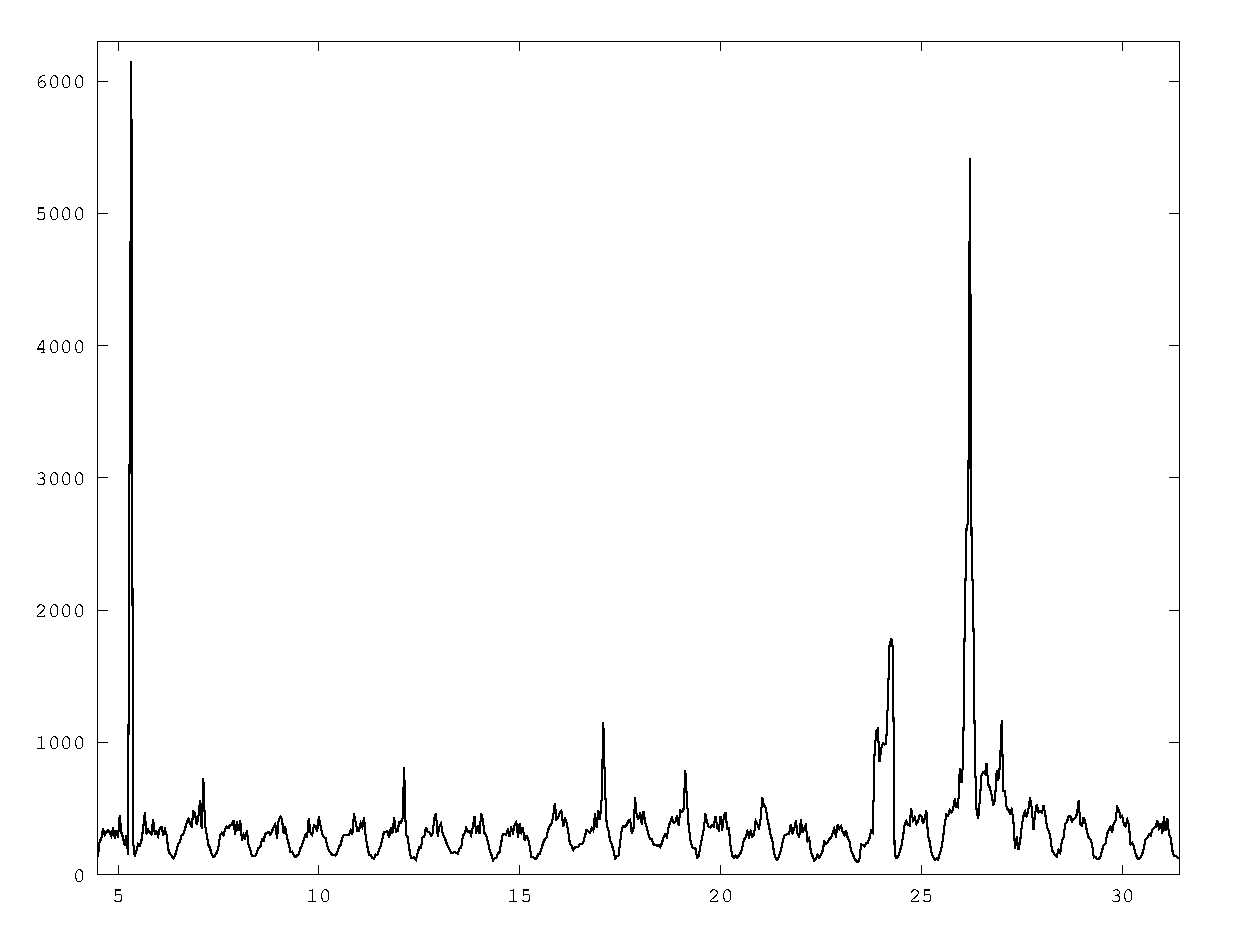
\includegraphics[width=7.5cm]{all-freq.eps}
  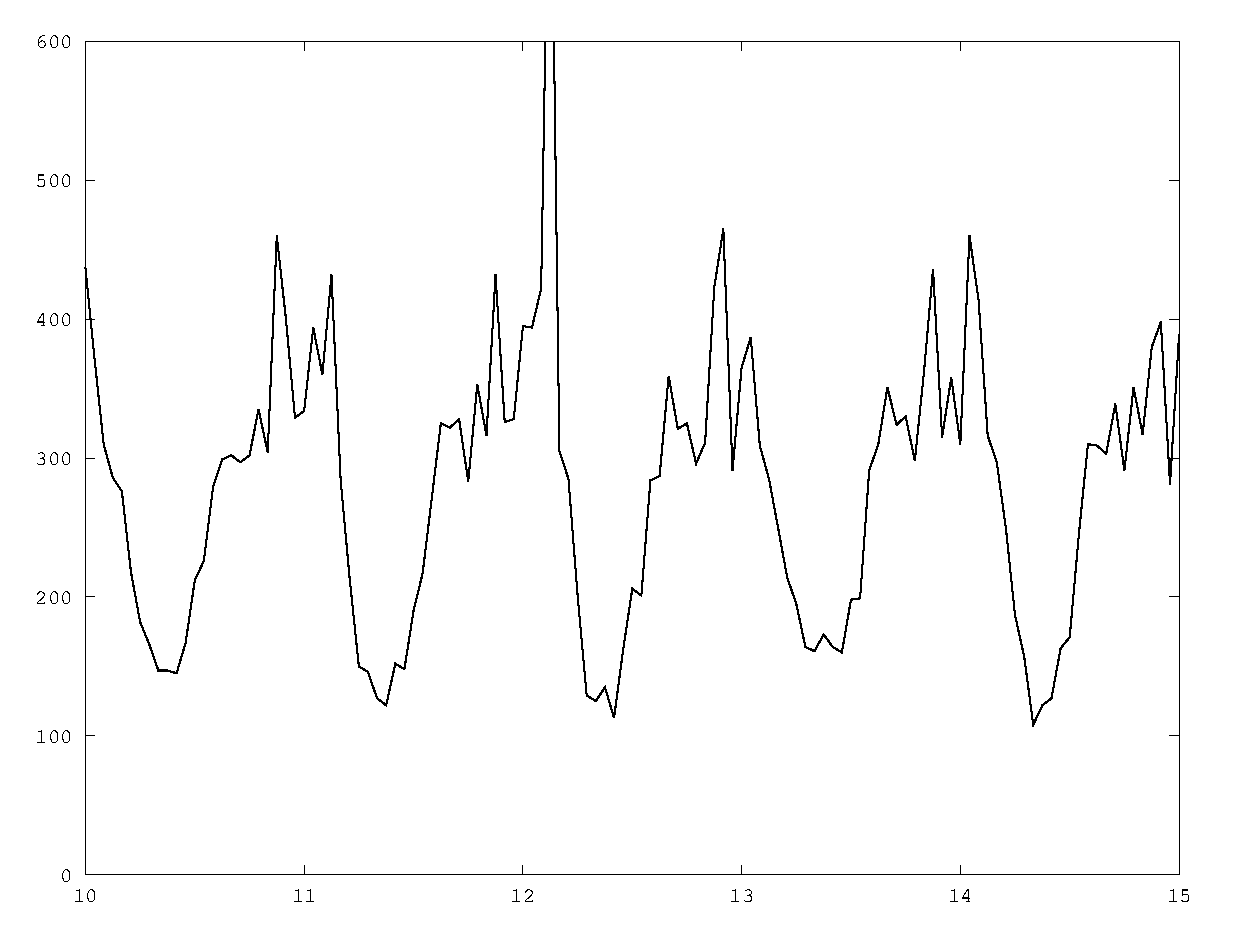
\includegraphics[width=7.5cm]{all-freq-scaled.eps}
  \caption{Зависимость количества сообщений в час от времени. На втором графике видна зависимость от времени суток.}
  \label{fig:all-freq}
  \end{figure}
  
  \subsection{Извлечение событий}
  
	На рисунке \ref{fig:all-freq-labeled} можно видеть экстремумы, отмеченные алгоритмом \ref{main-algo} на шаге \ref{alg:peaks-extraction}. Путем выбора метода и параметров, можно помечать больше или меньше максимумов. 

	 \begin{figure}[H]
	  \centering
	  \label{fig:all-freq-labeled}
	  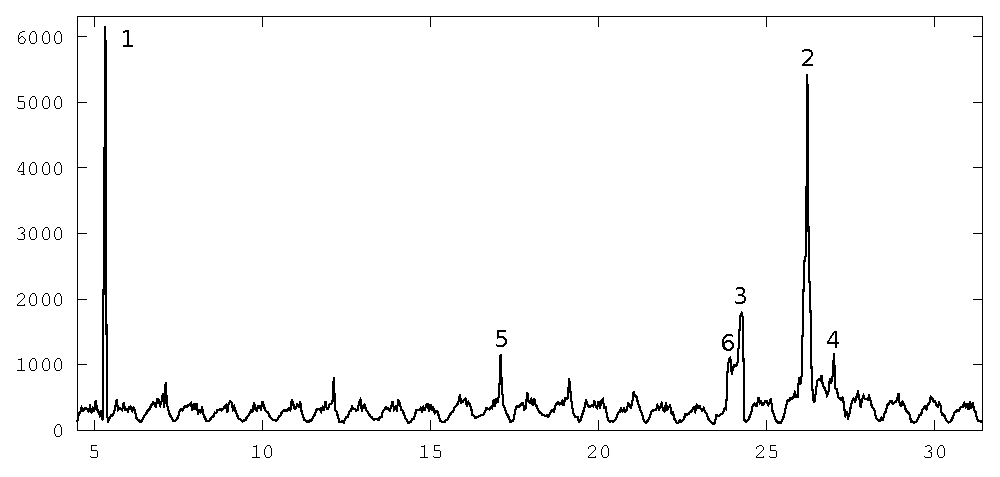
\includegraphics[width=15cm]{all-freq-labeled-1.eps}
	  \caption{График частоты сообщений с отмеченными экстремумами.}
	  \end{figure}
	  
	Следующие таблицы показывают параметры частотных характеристик сообщений, полученных на шаге \ref{alg:before-check} основного алгоритма. На основании этих данных те или иные события войдут в финальный результат или будут отброшены.
	
	\begin{table}[H]
	\centering
	\begin{tabular}{l | l}
	& $\sigma^2$ \\ 
	\#1 & 7853 \\ 
	\#2 & 8993 \\ 
	\#3 & 3500 \\ 
	\#4 & \textbf{34628} \\ 
	\#5 & \textbf{30232} \\ 
	\#6 & 4261 \\ 
	\end{tabular}
	\caption{Жирным шрифтом помечены события с $\sigma^2>\sigma_0^2$.}
	\label{sd-table}
	\end{table}
	
%\todo{triangle table}	
	
	\begin{table}[H]
	\centering
	\begin{tabular}{ r | c  c  c  c  c  c }
	\#1 & 1 &  &  &  &  &  \\ 
	\#2 & 0.004 & 1 &  &  &  &  \\ 
	\#3 & 0.001 & 0.009 & 1 &  &  &  \\ 
	\#4 & 0.057 & 0.109 & 0.131 & 1 &  &  \\ 
	\#5 & 0.038 & 0.079 & 0.120 & \textbf{0.935} & 1 &  \\ 
	\#6 & 0.001 & 0.006 & \textbf{1.000} & 0.132 & 0.121 & 1 \\ \hline
	& \#1 & \#2 & \#3 & \#4 & \#5 & \#6 \\
	\end{tabular}
	\caption{Значения нормализованного скалярного произведения функций частот в косинусной метрике. Жирным шрифтом помечены значения, позволяющие считать события тождественными.}
	\label{dotprod-table}
	\end{table}
	
	\begin{figure}[H]
	\centering

	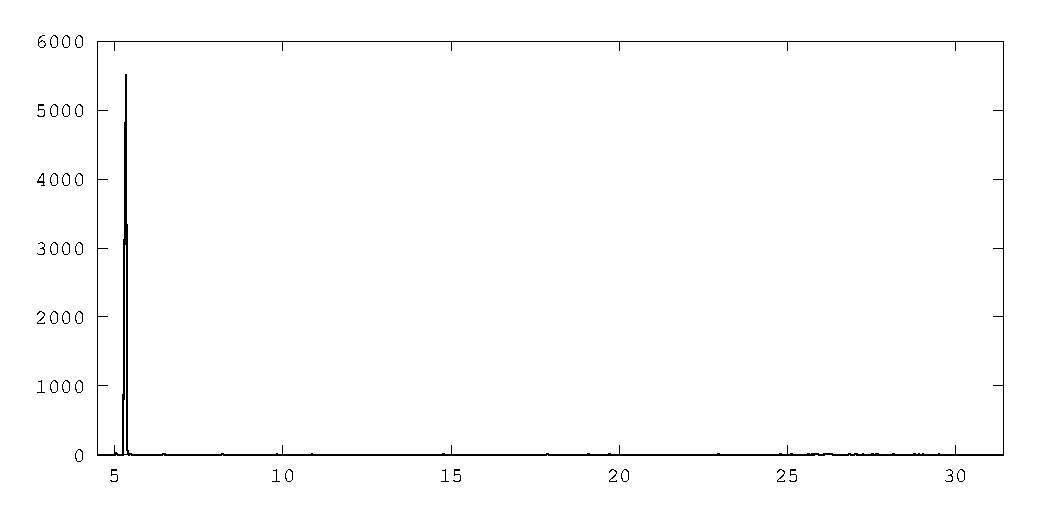
\includegraphics[width=7.5cm]{all-freq-5-8.eps}	
	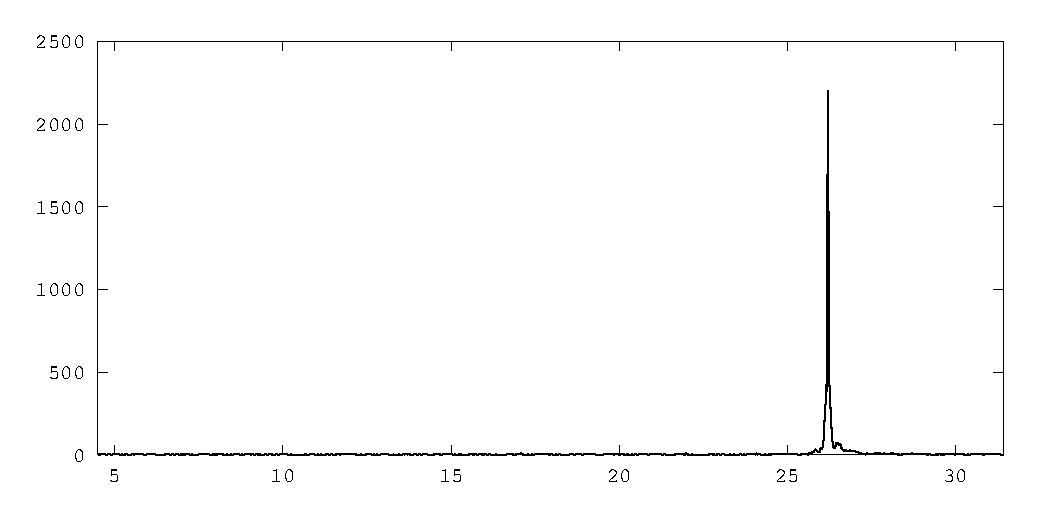
\includegraphics[width=7.5cm]{all-freq-26-5.eps}	
	
	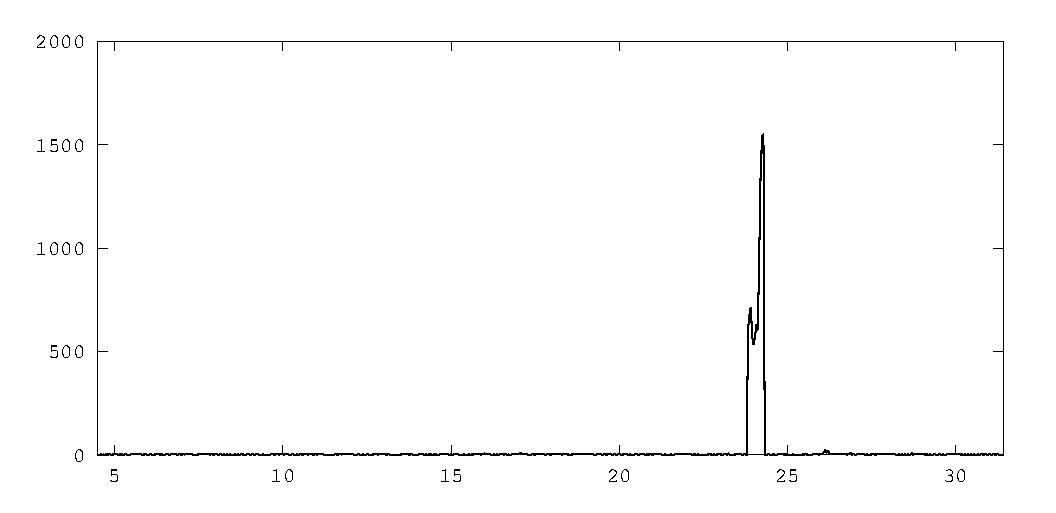
\includegraphics[width=7.5cm]{all-freq-24-6.eps}	
	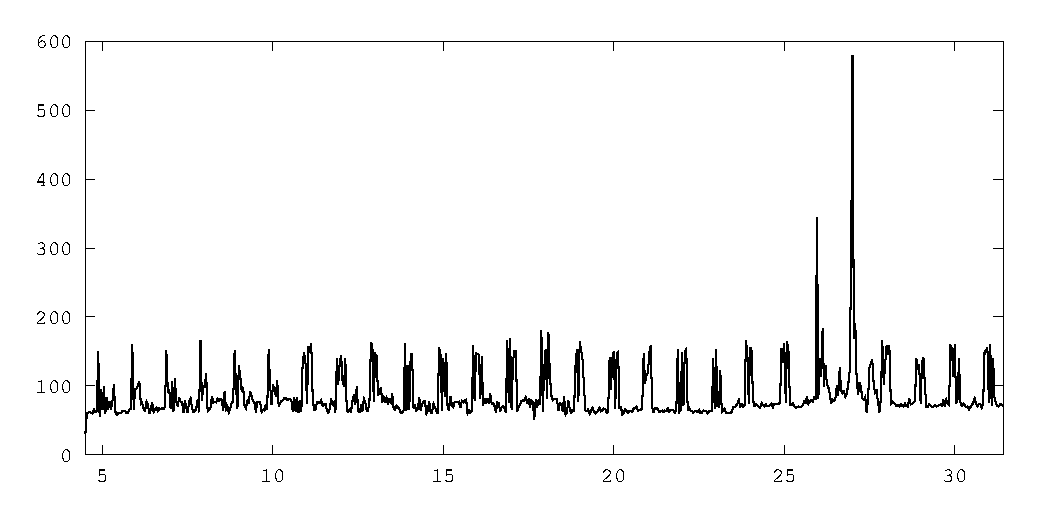
\includegraphics[width=7.5cm]{all-freq-27-0.eps}	
	
	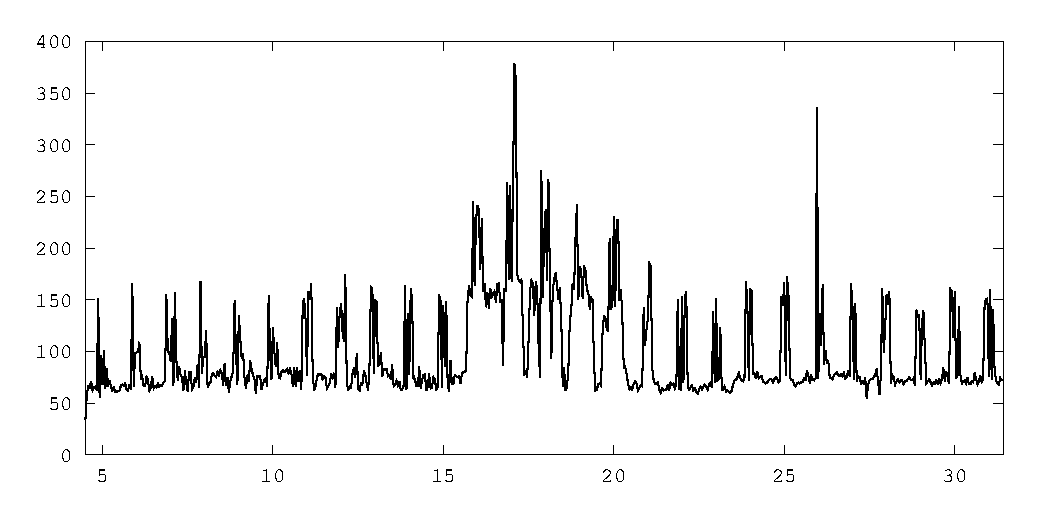
\includegraphics[width=7.5cm]{all-freq-17-2.eps}	
	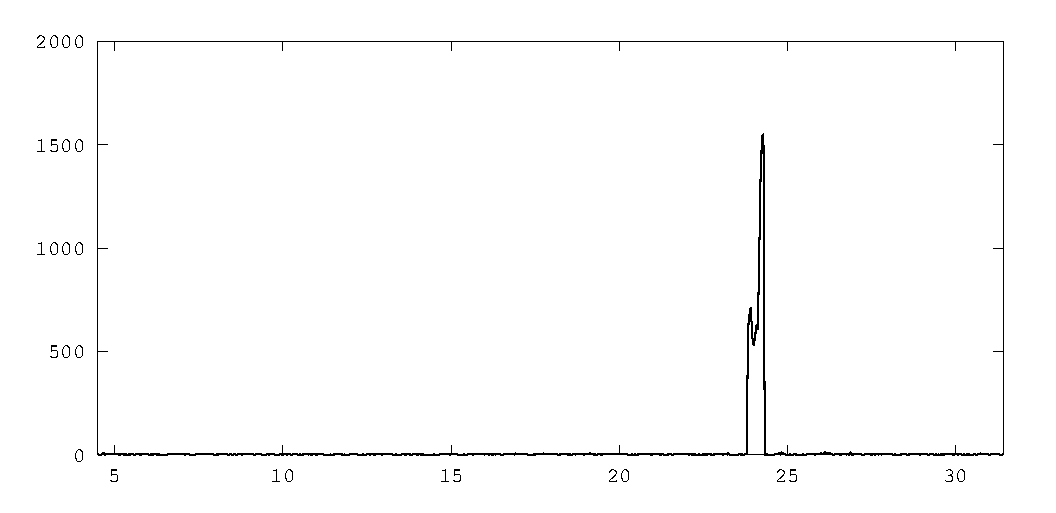
\includegraphics[width=7.5cm]{all-freq-23-20.eps}	
	
	\caption{Частоты сообщений для ``событий'' \#1 --- \#6.}
	\end{figure}
	
	Из таблиц \ref{sd-table} и \ref{dotprod-table} можно видеть, что алгоритм выдаст в конечном счете только события \#1, \#2, \#3. События \#4 и \#5 будут отброшены как имеющие большое среднеквадратичное отклонение. Событие \#6 не войдет в финальный результат потому, что значение похожести функций частоты для событий \#3, \#6 больше допустимой нормы:
\begin{equation}
	\simu^{\cos}(f_{\#3}, f_{\#6}) = \frac{(f_{\#3}, f_{\#6})}{ \Vert f_{\#3} \Vert \cdot \Vert f_{\#6} \Vert} > \theta_{\simu}.
\end{equation}

Приведем ниже таблицу \ref{event-table} с описаниями событий \#1, \#2, \#3:
	
	\begin{table}[H]
	\centering		
	\begin{tabular}{ l | l | l |}
	\hline
	 & Ключевые слова & Вызвавшее событие \\ \hline
	\#1 & \begin{tabular}{l} year, read, prison, dragon, \\ amazon, written, bestseller \end{tabular} & \begin{tabular}{l} Написанная в техасской тюрьме книга \\ The Sword and the Dragon является \\ бестселлером на Amazon уже более трех \\ лет. \end{tabular} \\ \hline
	\#2 & \begin{tabular}{l} sb5, standwithwendi, abort, \\ senat \end{tabular} & \begin{tabular}{l} Обсуждение сенатом закона по запрету \\ абортов, который носит название Senate \\ Bill 5. Wendi Davis ---  политик, которая \\ боролась с принятием этого закона.  \end{tabular} \\ \hline
	\#3 & \begin{tabular}{l} houston, california, england, \\ artist, rt, watch, defjam \end{tabular} & \begin{tabular}{l} Хип хоп исполнитель из Хьюстон Devin \\ the Dude объявил, что его восьмой \\ студийный альбом будет называться \\ One for the Road и будет выпущен в \\ продажу в сентябре 2013 года. Альбом \\ будет выпущен лейблом Def Jam \\ Recordings.\end{tabular} \\ \hline
	\end{tabular}
	
	\caption{Таблица с описаниями событий}
	\label{event-table}
	\end{table}
	
	Приведем значения параметров алгоритма \ref{main-algo}, при которых были полученны результаты этого раздела:
	
	\todo{Таблица с параметрами}
	
	\section{Заключение}
	В ходе выполения дипломной работы было достигнуто:
	\begin{itemize}
	\item изучены существующие методы извлечения и описания событий из коротких пользовательских сообщений,
	\item изучена возможность применения тематических моделей для это задачи,
	\item разработан и проанализирован алгоритм извлечения событий из социальной сети Твиттер на основе иерархического процесса Дирихле,
	\item алгоритм был реализован, параметры подобраны эксперементальным путем,
	\item тестирование показано, что алгоритм справляется с поставленной задачей.
	\end{itemize}
	
  
\begin{thebibliography}{9}
	\bibitem{nuggets}
	Imran, Elbassuoni, Castillo, Diaz and Meier.
	Extracting Information Nuggets from Disaster-Related Messages in Social Media.
	2013.
	\bibitem{waim13}
	Xun Wang, Feida Zhu, Jing Jiang, Sujian Li.
	Real Time Event Detection in Twitter.
	2011.
	\bibitem{ned}
	Thorsten Brants, Francine Chen, Ayman Farahat.
	A System for New Event Detection.
	2003.
	\bibitem{mediaeval}
	Konstantinos N. Vavliakis, Fani A. Tzima, and Pericles A. Mitkas.	
	Event Detection via LDA for the MediaEval2012 SED Task.
	2012.
	\bibitem{lda-model}
	David M. Blei, Andrew Y. Ng, Michael I. Jordan.
	Latent Dirichlet Allocation.
	2003.
	\bibitem{lda-gibbs}
	Tom Griffiths.
	Gibbs sampling in the generative model of Latent Dirichlet Allocation.
	\bibitem{peak-detection}
	Girish Keshav Palshikar.
	Simple Algorithms for Peak Detection in Time-Series.
	\bibitem{hdp-1}
	Yee Whye Teh, Michael I. Jordan, Matthew J. Beal, David M. Blei.
	Hierarchical Dirichlet Processes.
	2005.
	\bibitem{hdp-2}
	Yee Whye Teh.
	Hierarchical Bayesian Nonparametric Models with Applications.
	2009.
	\bibitem{ss-learning}
	Ramnath Balasubramanyan, William W. Cohen, Matthew Hurst.
	Modeling corpora of timestamped documents using semisupervised nonparametric topic models.
	\bibitem{blei-sd}
	 David Blei.
	 COS 424: Interacting with Data.
	 2008.
\end{thebibliography}
  
\end{document}
